\documentclass[12pt]{amsart}
\usepackage{geometry}                % See geometry.pdf to learn the layout options. There are lots.
 \geometry{
 a4paper,
 total={170mm,257mm},
 left=20mm,
 top=20mm,
 }
\usepackage{graphicx}
\usepackage{amssymb}
\usepackage{amsmath, amsthm}
\usepackage{epstopdf}
\usepackage{array}
\usepackage{url}
\usepackage{color}

\DeclareGraphicsRule{.tif}{png}{.png}{`convert #1 `dirname #1`/`basename #1 .tif`.png}

\newcolumntype{L}[1]{>{\raggedright\let\newline\\\arraybackslash\hspace{0pt}}m{#1}}
\newcolumntype{C}[1]{>{\centering\let\newline\\\arraybackslash\hspace{0pt}}m{#1}}
\newcolumntype{R}[1]{>{\raggedleft\let\newline\\\arraybackslash\hspace{0pt}}m{#1}}
\newcommand{\todo}[1]{{\color{red}$\blacksquare$~\textsf{[TODO: #1]}}}

\begin{document}

\noindent
\begin{tabular}{L{9.7cm} R{6.7cm}}
Astrophysical Radiation Processes: AS7005& Lab: 26.09.2022 \\
Evan O'Connor \& Yutong He & Due: 31.10.2022; on Athena\\
\end{tabular}\\

\vspace*{0.5cm}

\centerline{\Large \underline{Introduction to AS7005 Laboratory Exercise} }
\vspace*{0.5cm}

The purpose of this laboratory exercise is to solidify your
understanding of the fundamental radiation theory concept of
polarization, introduce you to some basic tools for radiation
transport, and get practice performing research, analysing results,
and writing scientifically.  These cover some of the learning outcomes
of the course, but also some of the learning outcomes of the Master's
program in general and is good preparation for the research project
later on in the degree program.  \newline

There is a prelab exercise (one of the standard weekly exercises) to
prep you for the content we will be looking at in the lab.  The lab
itself will be two parts.  The first will guide you through the
concepts of Thomson scattering, angular distributions, polarization,
Stokes parameters, and net polarization. Following this, the lab has
you perform Monto Carlo simulations of radiation transport with
photons from an aspherical supernovae in order to determine the net
polarization of the signal.  This will be the major work in the lab
session. The second part will be writing a paper-like lab report to
summarize the findings. Even though this research has been done before
(we'll see this below), when writing the report, please work under the
assumption you are doing this for the first time, typical for a
scientific paper. You can refer to the paper for the methods.  Please read
\mbox{\url{https://www.nature.com/articles/d41586-019-02918-5}} for
tips on writing scientifically.  \newline

For the paper please follow the outline below.  We suggest using
overleaf (\url{www.overleaf.com}), choose a new project with a
template, choose either ``Astronomy and Astrophysics'' or ``American
Astronomical Society''. Include an {\bf{Abstract}} summarizing the
paper and the findings.  An {\bf{Introduction}} where you give an
general overview of the astrophysical system we are modelling, and any
other background information needed for the paper. Include a summary
of the layout of the paper. Have a {\bf{Methods}} section where you
discuss briefly the theoretical model and methods (including a brief
description of the Monto Carlo transport).  Include key equations
(e.g., among others, the differential Thomson Scattering cross
section, $d\sigma/d\Omega$) and key derivations. It is fine if this is
more detailed that you would typically find in a research paper. Use
it show your understanding of the topic.  Have a {\bf{Results}}
section where you go through and present the verification of the Monte
Carlo simulations and the results of the net polarization study. End
with a {\bf{Conclusions}} section where you discuss and summarize the
results. Wrap things up with assessing what you think are the main
limitations of the methods (including sources of error) and possible
improvements.  \newline

The lab write up is intended to be done independently. But you are
encouraged to have discussions with each other and the lab instructors
during the lab itself, but please come to your own conclusions,
present your own data in your own plots, answer the questions on your
own, and submit your own paper. An A will be given for a well written
paper that follows the above outline, shows an excellent understanding
of the methods and results, and uses the tools of the lab to go
further in the analysis or to provide insight beyond what is
presented in the lab notebook. An acceptable lab report is required to
complete the course.  The lab component (the paper and the prelab
exercise) is 15\% of the total grade in the course. Please also save
the notebook and include in your submission a pdf copy of the jupyter
notebook you generated in the lab.  This will be especially useful
when you write up the lab, but also helps us with seeing your methods.

\newpage

\centerline{\Large \underline{Practicals for the Lab} }
\vspace*{0.5cm}



There is a git repository for this lab.
\url{https://github.com/evanoconnor/MCPolarization}. Download (or run
on \url{https://mybinder.org}).  Please read H\"oflich ``Asphericity
effects in scattering dominated photosphere'' A\&A 246 481
(1991). This paper is in the git repository in the {\tt {docs/}}
directory (as it this document).  The important parts of this paper
are the methods (Section 2) and results (Section 3), but not so much
the application to SN1987A (Section 4).  The purpose of the lab and
topic of your final paper is reproduce a selection of the results in
this paper.  Some methods and physical setups we use are different
from H\"oflich (1991), this is mainly for ease of implementation.  You
are more than welcome to enhance this work to include some of these
missing aspects, and please discuss with us your thoughts and we can
aide in your endeavour and make sure you doesn't forget any key
aspects. \newline

As we saw in the the prelab exercise, Thomson scattering
dominated atmospheres polarize the light coming from different
regions.  If the atmosphere is asymmetric than this can lead to an
asymmetry polarization signal, and ultimately a net polarization from
the source as a whole.  In this lab, we will construct such asymmetric
atmospheres and follow the trajectory of individual photons being
emitted from the origin.  Since the scattering will be due to Thomson
scattering, the polarization state of the photons depends on the
history of the photon.  If we simulate enough photons we can determine
the polarization pattern and the net polarization. \newline

The notebooks associated with this lab guide you through this whole
process.  Several key steps are missing, which will focus your
attention on the concepts relevant for this lab.  Please go through
the notebook slowly, read all the headers and comments and understand
what is happening. This part should take an hour or an hour and a
half.  By the end you should be able to reproduce Figure 7 of
H\"oflich (1991), reproduced below.  There are several lines on this
figure, our case most closely aligns with the dashed line (labeled \#1). \newline

\begin{figure}[h]
  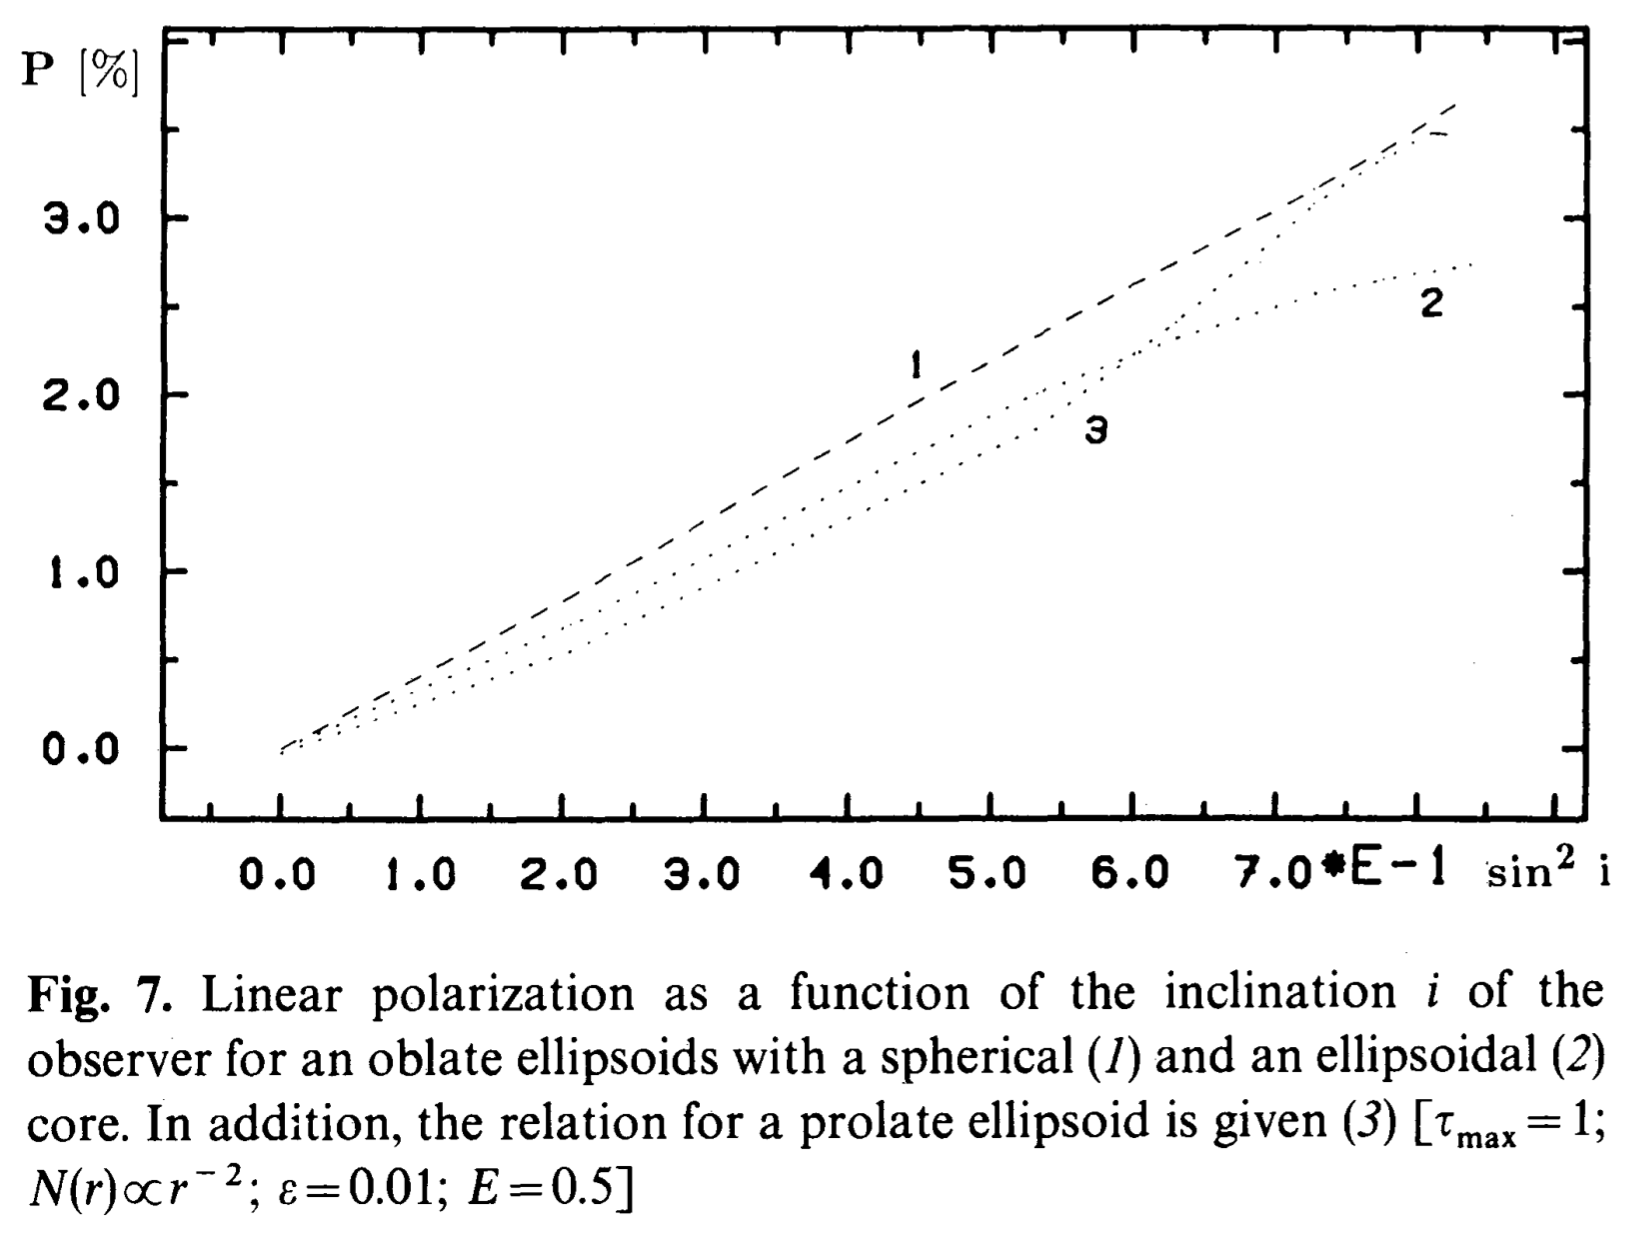
\includegraphics[width=0.5\textwidth]{hoeflich1991_fig7.png}
\end{figure}

For the remainder of the lab please design numerical experiments
exploring some of the other figures in H\"oflich (1991).  Some require
simply changing parameters, other require changing how routines are
designed.  We don't expect you to completely reproduce every figure,
but a few would be nice.  In addition to reproducing the figure,
please generate and include any figures that may help you explain the
methods and concepts in the paper.


\end{document}
